%% %%%%%%%%%%%%%%%%%%%%%%%%%%%%%%%%%%%%%%%%%%%%%%%%%
%% Template for a conference paper, prepared for the
%% Food and Resource Economics Department - IFAS
%% UNIVERSITY OF FLORIDA
%% %%%%%%%%%%%%%%%%%%%%%%%%%%%%%%%%%%%%%%%%%%%%%%%%%
%% Version 1.0 // November 2019
%% %%%%%%%%%%%%%%%%%%%%%%%%%%%%%%%%%%%%%%%%%%%%%%%%%
%% Ariel Soto-Caro
%%  - asotocaro@ufl.edu
%%  - arielsotocaro@gmail.com
%% %%%%%%%%%%%%%%%%%%%%%%%%%%%%%%%%%%%%%%%%%%%%%%%%%
\documentclass[11pt]{article}
\usepackage{UF_FRED_paper_style}
\usepackage{tabularx}
\usepackage{siunitx}
\usepackage{tipa}
\usepackage{textcmds}
\usepackage{multirow} 
%\usepackage{xcolor}
\usepackage[dvipsnames]{xcolor}
\usepackage{soul}
\definecolor{HLColor}{RGB}{230,230,250}
\sethlcolor{HLColor}
\usepackage[
    backend=biber,
    style=numeric,
  ]{biblatex}

\addbibresource{references.bib}
%% ===============================================
%% Setting the line spacing (3 options: only pick one)
%\doublespacing
% \singlespacing
\onehalfspacing
%% ===============================================
 
%\setlength{\droptitle}{-5em} %% Don't touch

% %%%%%%%%%%%%%%%%%%%%%%%%%%%%%%%%%%%%%%%%%%%%%%%%%%%%%%%%%%
% SET THE TITLE
% %%%%%%%%%%%%%%%%%%%%%%%%%%%%%%%%%%%%%%%%%%%%%%%%%%%%%%%%%%

% TITLE:
\title{\textbf{User Interface Design: Deliverable D1}\\Moodtracker for Companies}

% AUTHORS:
\author{Laurenz Kottek\\ Céline Nöhl\\ Alexandros Tsaparas\\ Noé Barbera}


    
% DATE:
\date{\today}

% %%%%%%%%%%%%%%%%%%%%%%%%%%%%%%%%%%%%%%%%%%%%%%%%%%%%%%%%%%
% %%%%%%%%%%%%%%%%%%%%%%%%%%%%%%%%%%%%%%%%%%%%%%%%%%%%%%%%%%
\begin{document}
% %%%%%%%%%%%%%%%%%%%%%%%%%%%%%%%%%%%%%%%%%%%%%%%%%%%%%%%%%%
% %%%%%%%%%%%%%%%%%%%%%%%%%%%%%%%%%%%%%%%%%%%%%%%%%%%%%%%%%%
% ABSTRACT
% %%%%%%%%%%%%%%%%%%%%%%%%%%%%%%%%%%%%%%%%%%%%%%%%%%%%%%%%%%
% %%%%%%%%%%%%%%%%%%%%%%%%%%%%%%%%%%%%%%%%%%%%%%%%%%%%%%%%%%
{\setstretch{.8}}
\maketitle 

\vspace{15mm}


\tableofcontents
\newpage


\section{Introduction to the Moodtracker}
In the following, the basic principle of the app is presented in order to be able to better classify all procedures and results of the user research and problem identification in the topic field.\\
The basic idea of our app is to uncover problems and grievances through regular anonymous surveys of employees and also to provide initial incentives and ideas on how to improve the working environment. Our Moodtracker app is specifically designed for companies interested in employee satisfaction. Survey results are provided to team leaders in a completely anonymous format. Employees can view their survey history and analyze how their answers have changed over time. In addition, there should still be a way for employees to contact their supervisors directly to communicate individual ideas and suggestions.
% --------------------
\section{Preparatory Research}
The following item deals with the relevance of our app as well as the user research. In particular, it discusses why employee satisfaction is important for companies. For this purpose, various scientific articles and publications as well as contributions from health-related organizations were considered. In addition, an exemplary survey was conducted in order to be able to specifically address user requirements when designing the app.
% --------------------
\subsection{Relevance of a Moodtracker for Companies}
In the course of our user research, we found numerous sources that prove that employee well-being is directly related to their productivity. For this reason, employee satisfaction and mental health is an increasingly important factor for companies.\\
The Saylor Academy is a nonprofit organization that offers free courses in many different areas, including management and leadership. One of their courses teaches the importance of an employee's mood \cite{noauthor_bus401_nodate}. They say, that the impact of a poor mood on decision-making can affect a person's job performance and lead to poor decisions that impact the organization. All moods can affect judgment, cognition, and physical and emotional well-being. Long-term exposure to negative moods or stressful environments can lead to illnesses such as heart disease, diabetes, and ulcers.\\
The publication \cite{inuwa_job_2016} analysed the relationship between employee satisfaction and performance. To this end, 270 non-academic employees of Bauchi State University Gadau Nigeria (BASUG) were surveyed. The result showed a significant relationship between satisfaction and productivity. This means that employees are more productive the more satisfied they are at their workplace.\\
Another paper \cite{chen_improving_2012} focussed on how conflict management in a company affects job satisfaction and innovation performance. To this end, 333 Chinese employees were surveyed. The study showed that integrating and compromising conflict management behaviour has positive effects on job satisfaction and innovation performance, while avoiding conflict management has negative effects.\\
Even the WHO explains in one of its articles that anxiety and bad mood can greatly reduce a team's productivity.\cite{noauthor_mental_nodate} For this reason, the WHO has developed tips and guides for employees and managers to protect and improve mental health in the working environment (\cite{WHO_guide_employee}, \cite{WHO_guide_policymakers}). Our application can be based on these guidelines and pass on some tips.\vspace{5mm} \\ 
To summarise, it can be said that employee satisfaction is extremely important for companies. It is therefore useful to obtain data on employee sentiment, as this can lead to solutions to improve the mood in the organization.\\
From our personal experience, it is known that in some companies, employees are often given forms asking them how they feel about certain things in the company. These forms are then given to supervisors to determine if some employees are having more problems than others.
Our application would solve the problem of automation and provide more data to work with.

\subsection{Survey as a Tool for User Research}
Our survey should help us identify the problems our application can solve and figure out how we can optimize its design to achieve the best result. We chose to design the survey as an open one, allowing participants to freely express their feedback and insights, broadening our perspective and encouraging open discussion.

\subsubsection{Realization of the Survey}
Due to the scope of our project, we have limited ourselves to a small number of participants. Nevertheless, we were able to gain the experience of doing a survey for user research and gain a good insight into how useful such a survey can be. Each of the three participants of the survey was asked three open questions. Some exemplary answers were provided for each question to enhance understanding of the question.
During the survey, the participants were asked the following questions and associated proposed answers:
\begin{enumerate}
  \item Which are existing problems at your workplace?
      \begin{itemize}
      \item teamwork
      \item explanation
      \item mental pressure
      \item communication
      \item ...
    \end{itemize}
  \item Which feedback options are already being used?
      \begin{itemize}
      \item feedback forms
      \item meetings
      \item psychological support
      \item ...
    \end{itemize}
  \item What kind of application can you think about, which could improve your work life?
      \begin{itemize}
      \item (anonymous) feedback app 
      \item chat
      \item motivational support 
      \item mood tracking
      \item filling in surveys/forms
      \item ...
    \end{itemize}
\end{enumerate}

\subsubsection{Results of the Survey}
While conducting the survey, we noticed that the open question format was unfavorable. The participants often had problems finding answers that related to the question. Nevertheless, we were able to gain some good insights and suggestions that are helpful for further design. The participants' answers are listed below. The answers most relevant to our project are highlighted.\\
\begin{enumerate}
  \item Existing Problems:
    \begin{itemize}
    \item not enough administrative rights
    \item \hl{lack of direct feedback}
    \item insufficient resources
    \item \hl{lack of communication}
    \item \hl{lack of regular satisfaction feedback}
    \item dependency on others without certainty
    \end{itemize}
    
  \item Existing Solutions:
    \begin{itemize}
    \item every three months surveys covering well-being,                      processes, and relationships with superiors
    \item feedback after resignations
    \item individual feedback to superiors
    \end{itemize}
    
  \item Possible Applications:
        \begin{itemize}
        \item creating a list to express concerns
        \item \hl{daily short feedbac}k on work satisfaction
        \item \hl{continuous feedback mechanisms}
        \item \hl{shared mindmap} where employees can leave positive and             negative feedback
        \end{itemize}
        
\end{enumerate}
The results of our survey showed that our app addresses precisely where there is currently room for improvement. Several respondents criticized the lack of feedback and suggested setting up a regular feedback format. In addition, the respondents do not yet have such regular feedback. The survey therefore confirms the need for a Moodtracker application to improve communication within the company and employee satisfaction.


% --------------------
\section{Key Problems}
% --------------------
Possible key problems with our app are presented and explained in detail below. The problems were categorized into problems that should be solved by future design and problems that arise through human-computer interaction.

\subsection{Problems to be Solved by Future Design}

\begin{description}
    \item[Trust] The trust of users in the app is one potential problem. In particular, the anonymization of the data could worry users, as they cannot be sure whether the data has really been anonymized correctly or whether it is possible to trace back if an employee gives bad feedback. This would have the consequence that the result of the surveys is better than it is in reality.
    \item[Honesty/ Seriousness] Another problem could be the way in which users answer the surveys. It is possible that some users do not take the surveys seriously and do not give accurate answers or are not completely honest and do not admit when they have a problem at work.
    \item[Visualization of the Survey Results] One problem that should be considered is the presentation of the survey results. Care must be taken to ensure that the results are easy to understand and clearly presented. At the same time, the results must not be distorted by the way they are presented. 
    \item[Questions and Answers] The nature of the question is another problem that needs to be considered. There are many different ways to collect data, such as multiple choice, single choice, or a slider or grading scale to agree with a statement. With the latter in particular, it should be noted that the user's answer can quickly contain a bias. On a grading scale, for example, the user will always tend towards the better grade. For this reason, the answer options in the sentiment survey must be chosen carefully. 
    \item[Limits of the Application] In addition to the points mentioned above, we must also bear in mind that our application has limitations. For example, an employee may have personal problems that go beyond the work environment. In this case, it is difficult for our app to identify the problem and provide assistance in finding a solution.
    \end{description}


% --------------------

\subsection{Possible HCI Problems}
\begin{description}
    \item[Simplicity of the App] The design of the app should be kept simple so that the user is not overwhelmed and can easily understand and use the app. If the structure of the application is too complicated, there is a risk that the user will lose patience and stop using the app and delete it. 

    \item[Problem of Persuasion] One design goal is to design the application in such a way that users are convinced to trust the app and its functionality and to use it seriously. The \ldq Trust\rdq and \ldq Honesty/ Seriousness\rdq points mentioned above encompass precisely this.
    
    \item[Visualization of Information] The problem of displaying information is a common problem. Here, for example, the above-mentioned points \ldq Visualization of the Survey Results\rdq and \ldq Questions and Answers\rdq are affected. The user must not be overwhelmed by too much information, but at the same time should be given a good overview of the most important information.
\end{description}


% --------------------
\printbibliography

\section{Appendix 1 - The survey as presented to the participants}
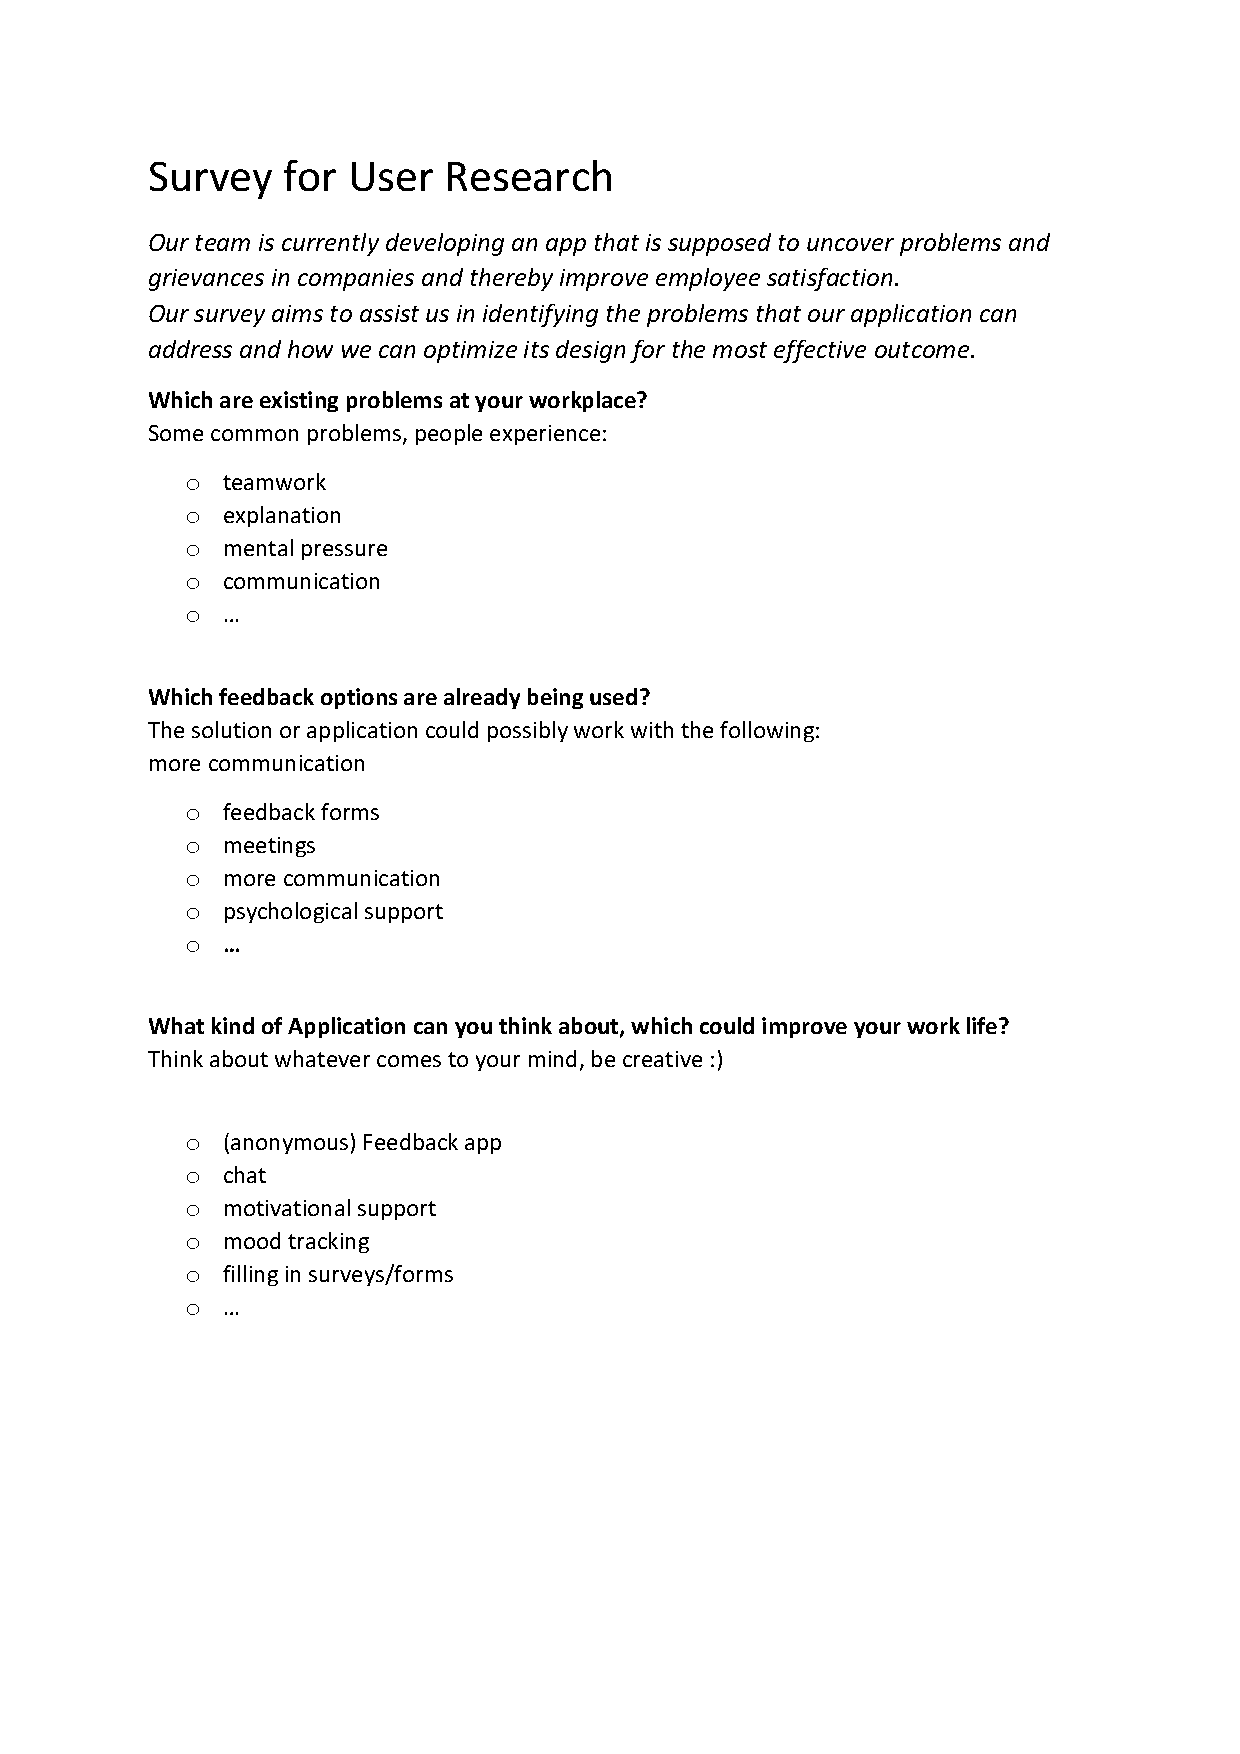
\includegraphics[height=\dimexpr\textheight-1\baselineskip\relax,page=1]{figures/UID - Survey 1 as Appendix.pdf}
% ==========================
% ==========================
% ==========================


\end{document}